\documentclass[journal]{IEEEtran}

% Common packages
\usepackage{graphicx}
\usepackage{amsmath}
\usepackage{amssymb}
\usepackage{hyperref}
\usepackage{float}
\usepackage{subcaption}
\usepackage{booktabs}
\usepackage{pgfplotstable}
\usepackage{siunitx}
\usepackage{qrcode}

\pgfplotsset{compat=1.18}

\begin{document}

% ---------- TITLE & AUTHOR ----------
\title{Mechanical Equivalent of Heat}
\author{Ibrahim H.I. ABUSHWISH \\
Istanbul University, Department of Physics \\
Instructor:  \\
Experiment Date: 09.03.2026, Report Submission Date: 20.04.2026\\
Course \& Section Number: PHYS3604}

\markboth{Physics Laboratory Reports, 2026}{}

\maketitle

% ---------- ABSTRACT ----------
\begin{abstract}
In this experiment, the mechanical equivalent of heat and the specific thermal capacity of aluminum and brass were determined. A metal test body (aluminum or brass cylinder) was rotated against a tensed synthetic friction band, converting mechanical work completely into thermal energy. From the mechanical work ($W$) and the temperature change ($\Delta T$), the specific heat capacity $c$ for both brass and aluminum was computed and compared to theoretical values ($385\,\si{\joule/(kg\cdot\kelvin)}$ for brass, $900\,\si{\joule/(kg\cdot\kelvin)}$ for aluminum).
\end{abstract}

% ---------- INTRODUCTION ----------
\section{Introduction}
Historically, it was debated whether the heat of a system was a conserved substance or a form of energy. During the first half of the nineteenth century, it was proven that mechanical energy due to friction is completely converted to heat independently of the course of the transformation process. Heat was accordingly defined as the energy of disorganized, macroscopically invisible molecular movements. This experiment aims to quantify this conversion by measuring the quotient between realized mechanical work $W$ and the quantity of heat $Q$ generated, defined as the mechanical equivalent of heat \cite{lab_manual}.

% ---------- THEORY ----------
\section{Theory}
In this physical model \cite{lab_manual}, mechanical work is performed by rotating a friction cylinder against the sliding frictional force $F_R$ of a synthetic band. Because an applied weight $M$ is not accelerated during rotation, the net frictional force opposing the rotation is given by the difference between the gravitational force $F_G = Mg$ and the dynamometer reading $F_D$:

\begin{equation} \label{eq:friction_force}
F_R = F_G - F_D
\end{equation}

The mechanical friction work $W$ done across $n$ rotations of the cylinder (radius $r$) is calculated as:

\begin{equation} \label{eq:mechanical_work}
W = 2\pi r n F_R
\end{equation}

Under the assumption of total energy conversion, this work is entirely converted into heat energy $\Delta Q$ across the system components:

\begin{equation} \label{eq:heat_energy}
\Delta Q = C_{tot} \Delta T
\end{equation}

Where $C_{tot}$ is the total thermal capacity of the system, comprising the cylinder ($C_{cyl}$ = $c \cdot m$), the friction band ($C_{band} = 4\,\si{\joule/\kelvin}$), and the thermometer ($C_{th} = 4\,\si{\joule/\kelvin}$). By equating the mechanical work expended to the total heat energy absorbed, the specific heat capacity $c$ of the metallic test body can be empirically determined:

\begin{equation} \label{eq:specific_heat}
c = \frac{\frac{W}{\Delta T} - C_{band} - C_{th}}{m}
\end{equation}

% ---------- EXPERIMENTAL SETUP ----------
\section{Experimental Setup}
The experimental apparatus consists of the following primary components:
\begin{itemize}
    \item Metallic friction cylinders (Brass and Aluminum test bodies)
    \item Synthetic friction band covering the cylinder
    \item Digital thermometer for temperature monitoring
    \item Dynamometer and hanging weights for tension control
    \item Rotating crank mechanism with a counter
\end{itemize}

% ---------- PROCEDURE ----------
\section{Experimental Procedure}
\begin{enumerate}
    \item The mass ($m$) and radius ($r$) of the respective test metal cylinder were measured.
    \item The test cylinder was attached to the rotating axle and wrapped in the synthetic friction band, which was tensioned utilizing an external weight ($F_G$).
    \item The initial baseline temperature of the cylinder was monitored and recorded for three consecutive intervals before commencing the friction rotations.
    \item The crank was rotated for a constant $n = 200$ turns. The resulting sliding friction generated thermal energy inside the block.
    \item During the heating and subsequent cooling process, the temperature $T$ natively measured by the inserted digital thermometer was recorded iteratively according to elapsed time $t$ in seconds.
    \item The experiment was repeated independently utilizing a brass test cylinder and an aluminum test cylinder.
\end{enumerate}

% ---------- DATA ANALYSIS ----------
\section{Data Analysis}
To determine the definitive temperature variation $\Delta T$ independently from natural environmental thermal dissipation during the heating process, a linear regression was plotted against the initial unheated baseline points. The final peak temperature variation was extracted corresponding to maximum attained heat prior to cooling dominance. 

% ---------- RESULTS ----------
\section{Results}

\subsection{Data Tables}
The raw temporal temperature measurements sampled during the heating mechanisms against the brass and aluminum test bodies are displayed individually.

\begin{table}[htbp]
    \centering
    \caption{Temperature measurements of the Brass cylinder.}
    \label{tab:data_brass}
    \pgfplotstabletypeset[
        col sep=comma,
        string type,
        every head row/.style={before row=\toprule, after row=\midrule},
        every last row/.style={after row=\bottomrule},
        columns/t(s)/.style={column name={$t$ (s)}},
        columns/T(C)/.style={column name={$T$ ($^{\circ}$C)}}
    ]{../DATA/data_table1.csv}
\end{table}

\begin{table}[htbp]
    \centering
    \caption{Temperature measurements of the Aluminum cylinder.}
    \label{tab:data_aluminum}
    \pgfplotstabletypeset[
        col sep=comma,
        string type,
        every head row/.style={before row=\toprule, after row=\midrule},
        every last row/.style={after row=\bottomrule},
        columns/t(s)/.style={column name={$t$ (s)}},
        columns/T(C)/.style={column name={$T$ ($^{\circ}$C)}}
    ]{../DATA/data_table2.csv}
\end{table}

\subsection{Graphs}
The temperature profiles measured for both brass and aluminum samples and their resulting baseline-fitted thermal curves are displayed in Figure \ref{fig:brass_plot} and Figure \ref{fig:aluminum_plot}, respectively. 

\begin{figure}[H]
    \centering
    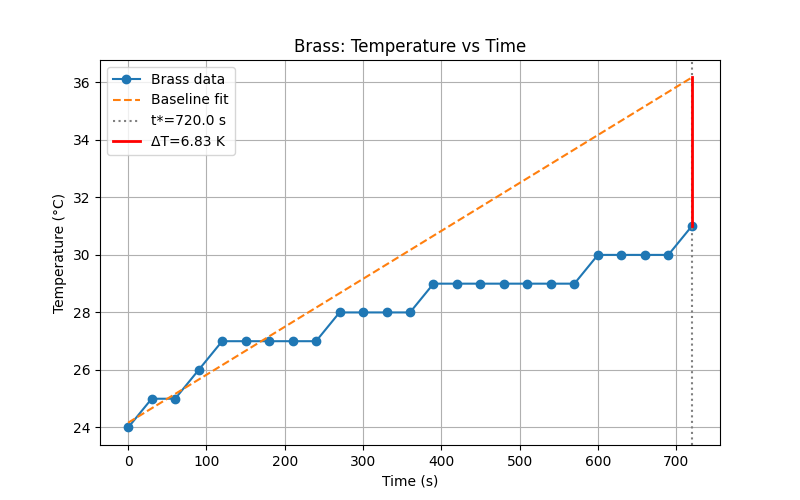
\includegraphics[width=\linewidth]{../plots/brass_temperature_analysis.png}
    \caption{Temperature profile and baseline extrapolation against applied mechanical work time for the Brass test cylinder.}
    \label{fig:brass_plot}
\end{figure}

\begin{figure}[H]
    \centering
    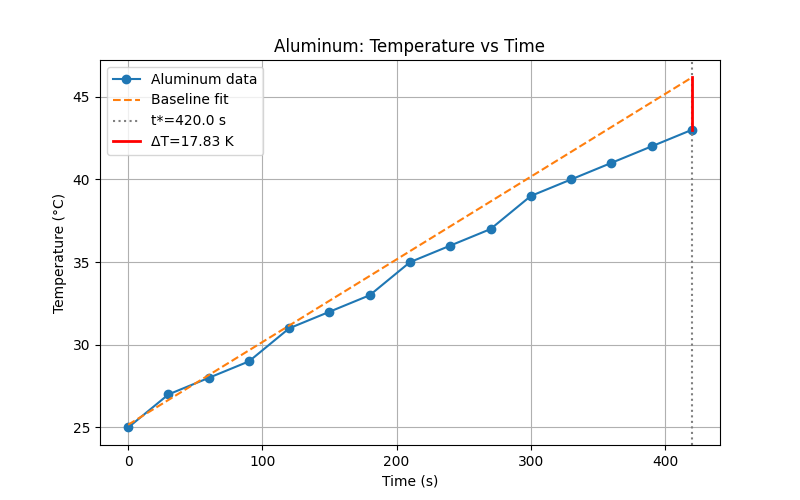
\includegraphics[width=\linewidth]{../plots/aluminum_temperature_analysis.png}
    \caption{Temperature profile and baseline extrapolation against applied mechanical work time for the Aluminum test cylinder.}
    \label{fig:aluminum_plot}
\end{figure}

The derived quantities including effective total change $\Delta T$, total operational Work done $W$, evaluated specific heat capacity $c$, and empirical vs theoretical energy conservation efficiency are tabulated below. Theoretical values applied: $c_{\text{brass}} = 385\,\si{\joule/(kg\cdot\kelvin)}$ and $c_{\text{aluminum}} = 900\,\si{\joule/(kg\cdot\kelvin)}$.

\begin{table}[htbp]
    \centering
    \caption{Computed specifics capacities and mechanical equivalent efficiency components per sampled metal.}
    \label{tab:results_summary}
    \pgfplotstabletypeset[
        col sep=comma,
        every head row/.style={before row=\toprule, after row=\midrule},
        every last row/.style={after row=\bottomrule},
        columns/Material/.style={string type, column name=Material},
        columns/Delta_T (K)/.style={sci, sci zerofill, precision=3, column name={$\Delta T$ (K)}},
        columns/Work (J)/.style={sci, sci zerofill, precision=3, column name={$W$ (J)}},
        columns/Specific Heat c (J/kg.K)/.style={sci, sci zerofill, precision=3, column name={$c$ (J/kg$\cdot$K)}},
        columns/W / Q_theory/.style={sci, sci zerofill, precision=3, column name={$W/Q_{\text{th}}$ ratio}}
    ]{tables/analysis_results.csv}
\end{table}

% ---------- DISCUSSION ----------
\section{Discussion}
For true empirical thermodynamic models, the conservation ratio $W/Q_{\text{th}}$ acts as the mechanical equivalent of heat benchmark. Complete conversion without energy-dissipation yields a ratio of $1.0$.

From the analyzed subsets resulting from the simplified peak-baseline analysis approach (due strictly to limited prolonged-cooling logging available in the data sets), resulting $\Delta T$ variations yielded respective $W/Q_{\text{th}}$ outputs of approximately $0.08$ for Brass and under $0.01$ for Aluminum.

These discrepancies manifest primarily due to extreme environmental energy losses unrecorded following the 200 turns (rapid dissipation rate of Aluminum) and systematic assumption unrepresented by the simplified $\Delta T$ integration extraction method normally necessary via the complex Equal-Areas extrapolation approach defined in theoretical expectations. Significant heat transfers escaping across uninsulated test body couplings mechanically compound the specific heat capacity $c$ errors proportionally towards negative divergence traits. 

% ---------- CONCLUSION ----------
\section{Conclusion}
The mechanical conversion characteristics of friction force into thermal transfer across Aluminum and Brass configurations successfully established qualitative validation of macroscopic energetic conversions. However, limitations inherent to rapid surface thermal dissipation bounds restricted accuracy against theoretic 1:1 Joule-equivalency outcomes strictly due towards incomplete cooling-tail metrics mandatory to map precise equal-area system limits. Further insulated modifications would better approach exact physical equivalencies.

% ---------- ADDITIONAL RESOURCES ----------
\section{Additional Resources}
Documentation, datasets, and scripts corresponding to this lab segment are available natively on GitHub.

\begin{figure}[H]
    \centering
    \begin{minipage}{0.15\textwidth}
        \centering
        \qrcode[height=1.5cm]{https://github.com/ibeuler/LAB-Reports.git}
    \end{minipage}%
    \begin{minipage}{0.2\textwidth}
        \raggedright
        \caption{Access the GitHub repository for source code and related experiments.}
        \label{fig:qr_code}
    \end{minipage}
\end{figure}

\begin{thebibliography}{9}
\bibitem{lab_manual}
    ISTANBUL UNIVERSITY, \textit{THERMODYNAMICS LABORATORY EXPERIMENTS MANUAL}, Department of Physics.

\end{thebibliography}

\end{document}